\documentclass[a4paper, 11pt]{article}

\usepackage[utf8]{inputenc}
\usepackage[english]{babel}

\usepackage{hyperref}

\usepackage{graphicx}
\usepackage{float}
\usepackage{tikz}

\usepackage{listings}

\usepackage{fullpage}

\begin{document}
	\begin{centering}
		\Large{\textbf{Progress Report}}\\
		\large{\today}
~\\
		Oussama ENNAFII\\
		Directors: Cl\'ement Mallet \& Florent Lafarge \\
		Advisor: Arnaud Le Bris \\

	\end{centering}


	\section{The Dataset:}
~\\

	We have decided earlier in June to work on Nantes and Dijon in addition to
	Elancourt. As I explained later, the $3DS$ data for these regions are not
	well formated so that I can retrieve the building entities. In order to
	establish first a whole pipeline. I will deal with those regions later using
	the $CityGML$ data. In consequence, I will continue to work on Elancourt
	only, for now.\\

	I have also relabelled the zone I had labelled before. That is due to the fact
	that the taxonomy has evolved during the annotation. I have used $QGIS$ to
	annotate buildings' projected facets based on errors they showed.\\

	The errors have been subdivided, based on the labelling, into three classes:

	\begin{itemize}
		\item[-] Unqualified Building Errors: Concerns the buildings that will not
		be taken into consideration,
		\item[-] Building Errors: encompasses the errors that affect the whole
		building (corrensponds roughly to $LoD0$ and $LoD1$ errors),
		\item[-] Facet Errors: concerns errors affecting only a facet.
	\end{itemize}

	\begin{figure}[H]
		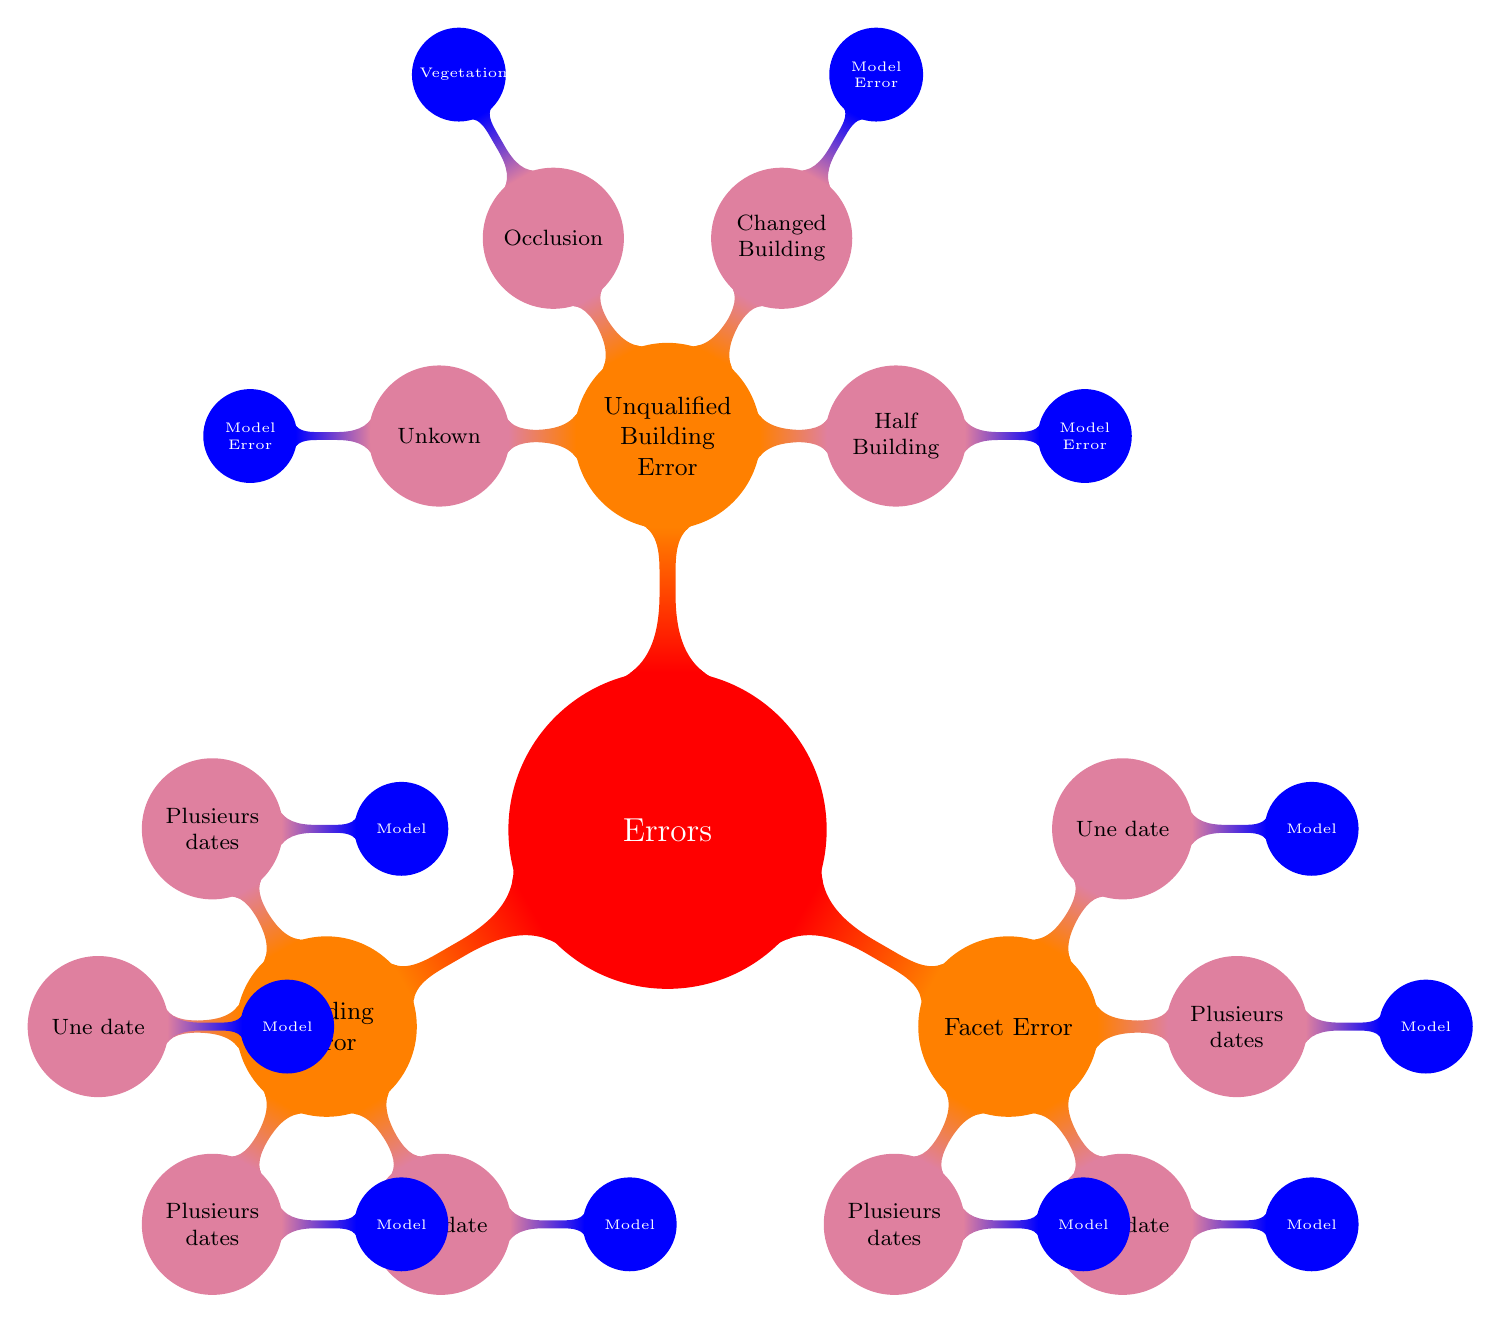
\begin{tikzpicture}
			\usetikzlibrary{mindmap, trees}
			\path[mindmap, concept color=red, text=white]
				node[concept]{Errors}[clockwise from=0]
				child[concept color=orange, text=black, grow=90]
				{
					node[concept]{Unqualified Building Error}[clockwise from=0]
					child[concept color=purple!50, text=black, grow=0]
					{
						node[concept]{Half Building}[clockwise from=0]
						child[concept color=blue, text=white, grow=0]
						{
							node[concept]{Model Error}
						}
					}
					child[concept color=purple!50, text=black, grow=60]
					{
						node[concept]{Changed Building}[clockwise from=0]
						child[concept color=blue, text=white, grow=60]
						{
							node[concept]{Model Error}
						}
					}
					child[concept color=purple!50, text=black, grow=120]
					{
						node[concept]{Occlusion}
						child[concept color=blue, text=white, grow=120]
						{
							node[concept]{Vegetation}
						}
					}
					child[concept color=purple!50, text=black, grow=180]
					{
						node[concept]{Unkown}
						child[concept color=blue, text=white, grow=180]
						{
							node[concept]{Model Error}
						}
					}
				}
				child[concept color=orange, text=black, grow=330]
				{
					node[concept]{Facet Error}
					child[concept color=purple!50, text=black, grow=60]
					{
						node[concept]{Une date}
						child[concept color=blue, text=white, grow=0]
						{
							node[concept]{Model}
						}
					}
				  child[concept color=purple!50, text=black, grow=0]
					{
						node[concept]{Plusieurs dates}
						child[concept color=blue, text=white, grow=0]
						{
							node[concept]{Model}
						}
					}
					child[concept color=purple!50, text=black, grow=300]
					{
						node[concept]{Une date}
						child[concept color=blue, text=white, grow=0]
						{
							node[concept]{Model}
						}
					}
				  child[concept color=purple!50, text=black, grow=240]
					{
						node[concept]{Plusieurs dates}
						child[concept color=blue, text=white, grow=0]
						{
							node[concept]{Model}
						}
					}
				}
				child[concept color=orange, text=black, grow=210]
				{
					node[concept]{Building Error}
					child[concept color=purple!50, text=black, grow=300]
					{
						node[concept]{Une date}
						child[concept color=blue, text=white, grow=0]
						{
							node[concept]{Model}
						}
					}
				  child[concept color=purple!50, text=black, grow=240]
					{
						node[concept]{Plusieurs dates}
						child[concept color=blue, text=white, grow=0]
						{
							node[concept]{Model}
						}
					}
					child[concept color=purple!50, text=black, grow=180]
					{
						node[concept]{Une date}
						child[concept color=blue, text=white, grow=0]
						{
							node[concept]{Model}
						}
					}
				  child[concept color=purple!50, text=black, grow=120]
					{
						node[concept]{Plusieurs dates}
						child[concept color=blue, text=white, grow=0]
						{
							node[concept]{Model}
						}
					}
				};
		\end{tikzpicture}
		\caption{\label{fig::mindmap_errors} Mind map representing the errors encountered during the annotation.}
\end{figure}

\section*{Attachments:}

\begin{itemize}
	\item[-] You can checkout the preprocessing code on
	\href{https://github.com/ethiy/proj.city}{Github}.
	\item[-] You can also check the feature extraction and classification code
	\href{https://github.com/ethiy/qualcity}{here}.
\end{itemize}

\end{document}
